\documentclass[12pt,a4paper]{article}
\usepackage[UTF8]{ctex}
\usepackage{geometry}
\usepackage{graphicx}
\usepackage{float}
\usepackage{amsmath}
\usepackage{amsfonts}
\usepackage{amssymb}
\usepackage{booktabs}
\usepackage{multirow}
\usepackage{array}
\usepackage{longtable}
\usepackage{enumerate}
\usepackage{fancyhdr}
\usepackage{lastpage}
\usepackage{hyperref}
\usepackage{siunitx}
\usepackage{wrapfig}
\usepackage{caption}
\usepackage{enumitem}

% 页面设置
\geometry{left=2.5cm,right=2.5cm,top=2.5cm,bottom=2.5cm}

% 行距设置
\linespread{1.2}

% 段落缩进
\setlength{\parindent}{2em}

% 修复页眉高度问题
\setlength{\headheight}{14.49998pt}
\addtolength{\topmargin}{-2.49998pt}

% 页眉页脚设置
\pagestyle{fancy}
\fancyhf{}
\fancyhead[C]{实\hspace{0.5em}验\hspace{0.5em}报\hspace{0.5em}告}
\fancyfoot[C]{\thepage}

\begin{document}

% 正文第一行标题
\noindent
{\Large \textbf{实验十一：}\underline{\textbf{串联谐振电路}}} \hfill {\Large \textbf{实验成绩：}\underline{\hspace{3cm}}}
\vspace{0.5cm}

\section*{一、实验目的}
\begin{enumerate}
    \item 观察串联电路谐振现象，加深对谐振条件和特点的理解。
    \item 学习 RLC 串联谐振电路频率特性曲线的测定方法。
\end{enumerate}

\section*{二、实验原理}

\begin{enumerate}
        \item \textbf{串联谐振电路的幅频特性和相频特性}
    
    \noindent
    \begin{minipage}[c]{0.58\textwidth}
        RLC串联电路如图所示，其入端阻抗为：
        \[ Z = R + j\left(\omega L - \dfrac{1}{\omega C}\right) = \lvert Z \rvert\angle\phi \]
        
        当$ \omega_0 L - \dfrac{1}{\omega_0 C} = 0 $时，电路达到谐振状态，此时的谐振角频率为：
        \[ \omega_0 = \dfrac{1}{\sqrt{LC}} \]
        
        谐振频率为：$ f_0 = \dfrac{\omega_0}{2\pi} $。
        
        谐振时，电路的阻抗为$ Z = R $，电路的电流达到最大值$ I_0 = \dfrac{U}{R} $。
    \end{minipage}%
    \hfill
    \begin{minipage}[c]{0.38\textwidth}
        \centering
        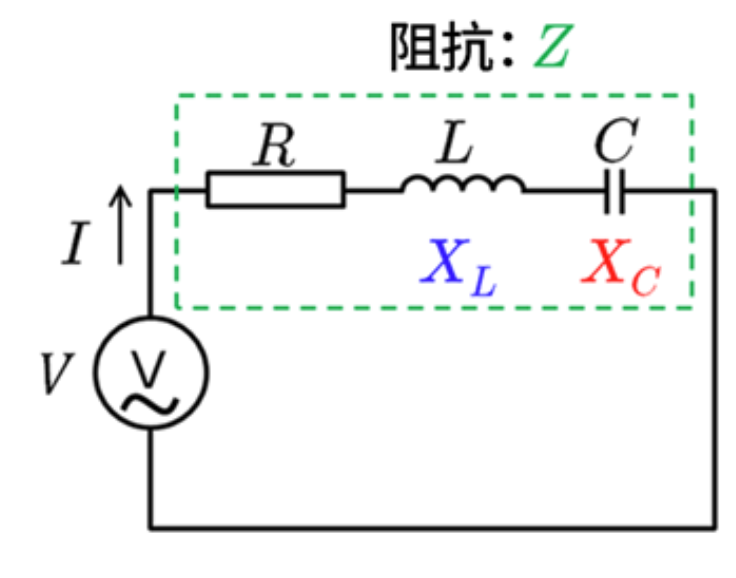
\includegraphics[width=\textwidth]{E11/RLC.png}
        \captionof{figure}{幅频特性和相频特性}
    \end{minipage}
    
    \item \textbf{串联谐振电路的幅频特性和相频特性}
    
    \[ I = \dfrac{U}{\sqrt{R^2 + (\omega L - \dfrac{1}{\omega C})^2}} = \dfrac{U}{R\sqrt{1 + Q^2(\dfrac{\omega}{\omega_0} - \dfrac{\omega_0}{\omega})^2}} \]
    
    其中$ Q = \dfrac{\omega_0 L}{R} = \dfrac{1}{\omega_0 CR} $为电路的品质因数。
    
    令$ \frac{U_s}{R} = I。 $，则$ \dfrac{I}{I_0} = \dfrac{1}{\sqrt{1 + Q^2(\dfrac{\omega}{\omega_0} - \dfrac{\omega_0}{\omega})^2}} $。
    
    $\dot{I}$与$\dot{U_s}$的相位差为：
    \[ \phi = \tan^{-1}(\dfrac{\omega L - \dfrac{1}{\omega C}}{R}) = \tan^{-1}(Q(\dfrac{\omega}{\omega_0} - \dfrac{\omega_0}{\omega})) \]
    
    两个频率$ \left( \frac{\omega_2}{\omega_0}, \frac{\omega_1}{\omega_0}\right)$ 之间的区域为相对同频带宽度$ \beta = \dfrac{\omega_2 - \omega_1}{\omega_0} $。
    \begin{figure}[H]
    \centering
    
\includegraphics[width=1\textwidth]{E11/frequency_response.png}
    \caption{串联谐振电路的幅频特性和相频特性}
    \end{figure}

\end{enumerate}

\section*{三、思考题}
\begin{enumerate}

    \item 在如图 7-19 所示的实验电路中,发生谐振时是否满足关系$ u_R = u_s, u_C = u_L $? 若关系不成立,请分析原因,并计算电感的等效内阻。
    
\begin{figure}[H]
    \centering
    
\includegraphics[width=0.6\textwidth]{E11_preview/schematic.png}
    \caption{图7-9}
    \label{fig:nonlinear_resistor_va}
\end{figure}
    
    \textbf{解：}关系不完全成立。
    
    \textbf{理论分析：}
    
    在理想串联谐振电路中，谐振时应满足：
    \begin{itemize}
        \item $X_L = X_C$，即 $\omega_0 L = \dfrac{1}{\omega_0 C}$
        \item $u_C = u_L$（电容和电感电压大小相等，相位相反）
        \item $u_R = u_s$（电阻电压等于电源电压）
    \end{itemize}
    
    但实际电路中，电感线圈存在直流电阻 $R_L$（等效内阻），实际阻抗应为：
    \[ Z = R + R_L + j\left(\omega L - \dfrac{1}{\omega C}\right) \]
    
    谐振时，虽然感抗与容抗相等，但总阻抗为 $Z = R + R_L$，因此：
    \[ u_R \neq u_s \]
    
    \textbf{计算电感等效内阻：}
    
    由实验数据：$f_0 = 1362$ Hz，$I_0 = 10.96$ mA
    
    设电源电压峰峰值为 $u_{spp}$，
    
    谐振时总阻抗：
    \[ R_{total} = R + R_L = \dfrac{u_s}{I_0} \]
    
    已知 $R = 510$ Ω，理论品质因数 $Q = 1.32$：
    \[ Q = \dfrac{\omega_0 L}{R + R_L} \Rightarrow R + R_L = \dfrac{\omega_0 L}{Q} \]
    
    由 $Q = 1.32$，$L = 0.1$ H，$f_0 = 1362$ Hz：
    \[ R + R_L = \dfrac{2\pi \times 1362 \times 0.1}{1.32} = 645 \text{ Ω} \]
    
    因此电感等效内阻：
    \[ R_L = 645 - 510 = 135 \text{ Ω} \]
    

    \item 可采用哪些实验方法判断电路是否已达串联谐振状态?
    
    \textbf{解：}可采用以下几种实验方法：
    
    \begin{enumerate}[label=(\arabic*)]
        \item \textbf{电流最大法：}
        
        调节信号源频率，观察电路电流，当电流达到最大值时，电路达到谐振状态。这是最直接、最常用的方法。
        
        \item \textbf{相位法：}
        
        使用双踪示波器同时观察电源电压 $u_s(t)$ 和电流 $i(t)$（或电阻两端电压 $u_R(t)$）的波形。当两波形同相位（相位差为零）时，电路达到谐振。
        
        \item \textbf{电压法：}
        
        测量电容或电感两端的电压，当其达到最大值时（$u_C = u_L = Q \cdot u_s$），电路谐振。
        
        \item \textbf{阻抗最小法：}
        
        测量电路总阻抗 $Z$，当阻抗最小（$Z = R$）时，电路谐振。
        
        \item \textbf{功率因数法：}
        
        测量功率因数 $\cos\phi$，当功率因数为 1（即 $\phi = 0$）时，电路达到谐振。
        
        \item \textbf{频率扫描法：}
        
        使用频率扫描功能，绘制幅频特性曲线，曲线峰值对应的频率即为谐振频率。
    \end{enumerate}

    \item 某同学根据 RLC 串联谐振电路参数计算出,理论谐振频率为 356 Hz,而实验测得为 330 Hz,请分析主要误差来源。
    
    \textbf{解：}理论值与实验值存在约 7.3\% 的偏差，主要误差来源包括：
    
    \begin{enumerate}[label=(\arabic*)]
        \item \textbf{电感参数误差：}
        
        电感的标称值与实际值存在偏差，电感线圈的电感量受温度、频率影响，实际电感可能与标称值不符。
        
        \item \textbf{电容参数误差：}
        
        电容的实际容量可能与标称值有偏差，电容的容值也会随温度和频率变化。
        
        \item \textbf{分布参数影响：}
        
        电路中存在分布电容和分布电感，特别是导线、电感线圈的分布电容会使实际谐振频率降低。
        
        \item \textbf{电感线圈损耗：}
        
        电感的等效串联电阻 $R_L$ 会影响谐振频率，特别是当 $R_L$ 较大时，实际谐振频率为：
        \[ f_0' = f_0 \sqrt{1 - \dfrac{R_L^2 C}{L}} < f_0 \]
        
        \item \textbf{测量误差：}
        
        频率测量仪器的精度限制、读数误差等。
        
        \item \textbf{负载效应：}
        
        测量仪器（如示波器探头）的输入阻抗和电容会影响电路参数。
    \end{enumerate}
    
    \textbf{改进建议：}使用精密仪器测量元件实际参数，考虑分布参数影响，使用修正公式计算。
    
    \item 试利用谐振原理,使用已知标准电容设计测量未知电感的实验方案。
    
    \textbf{解：}基于串联谐振原理的电感测量方案：
    
    \textbf{实验原理：}
    
    串联谐振时，谐振频率与电感、电容的关系为：
    \[ f_0 = \dfrac{1}{2\pi\sqrt{LC}} \]
    
    因此，未知电感可表示为：
    \[ L = \dfrac{1}{(2\pi f_0)^2 C} \]
    
    \textbf{实验步骤：}
    
    \begin{enumerate}[label=\arabic*.]
        \item 将待测电感 $L_x$、标准电容 $C_0$（已知精确值）、小电阻 $R$ 和信号源串联组成谐振电路。
        
        \item 调节信号源频率，观察电路电流或电阻两端电压。
        
        \item 当电流达到最大值（或 $u_R$ 最大）时，记录此时的频率 $f_0$，即为谐振频率。
        
        \item 使用示波器验证电压与电流同相，确认达到谐振。
        
        \item 根据公式计算待测电感：
        \[ L_x = \dfrac{1}{4\pi^2 f_0^2 C_0} \]
        
        \item 为提高精度，可使用不同的标准电容重复测量，取平均值。
    \end{enumerate}
    
    \textbf{注意事项：}
    \begin{itemize}
        \item 选择高精度标准电容（误差 $\leq 1\%$）
        \item 电阻 $R$ 应较小，以获得较高的品质因数和明显的谐振现象
        \item 考虑电感线圈内阻的影响
        \item 使用频率计精确测量谐振频率
    \end{itemize}
    
\end{enumerate}

\section*{四、实验任务与线路}
\begin{enumerate}
    \item 找出 RLC 串联谐振的谐振点,记录谐振频率 $f_0$,串联测量谐振点电流 $I_0$,并绘出此时端口电压 $u_s(t)$ 和电流 $i(t)$ 的波形。

    \item 测量 RLC 谐振电路的幅频特性(可以用示波器的自动测量)。

    \item 测量 RLC 谐振电路的相频特性(可以用示波器的自动测量)。
\end{enumerate}

\section*{五、实验数据记录与分析}

\begin{itemize}
    \item 谐振点：$ f_0 = 1362 Hz, I_0 = 10.96 mA $

\begin{figure}[H]
    \centering
    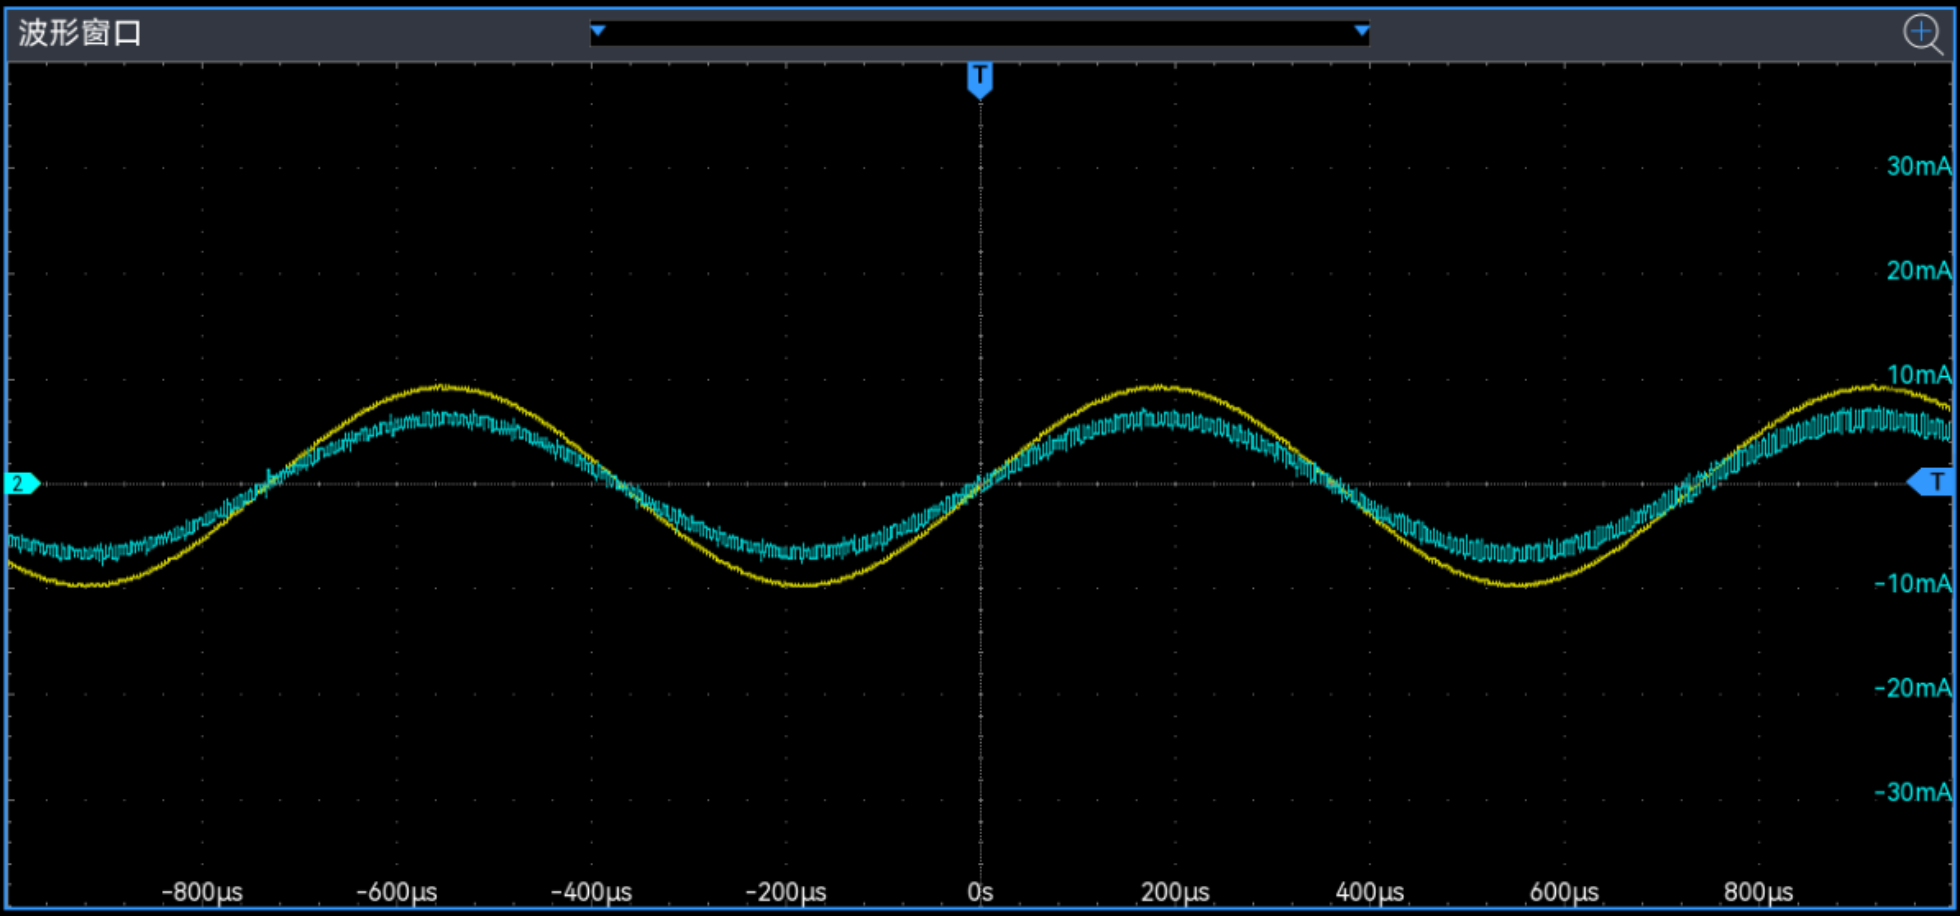
\includegraphics[width=0.8\textwidth]{../picture/1.png}
    \caption{谐振点端口电压和电流波形}
\end{figure}
    \item 由波形图可以看出，此时电压与电流相位相同，符合发生谐振的特性。
\end{itemize}


    \begin{figure}[H]
        \centering
        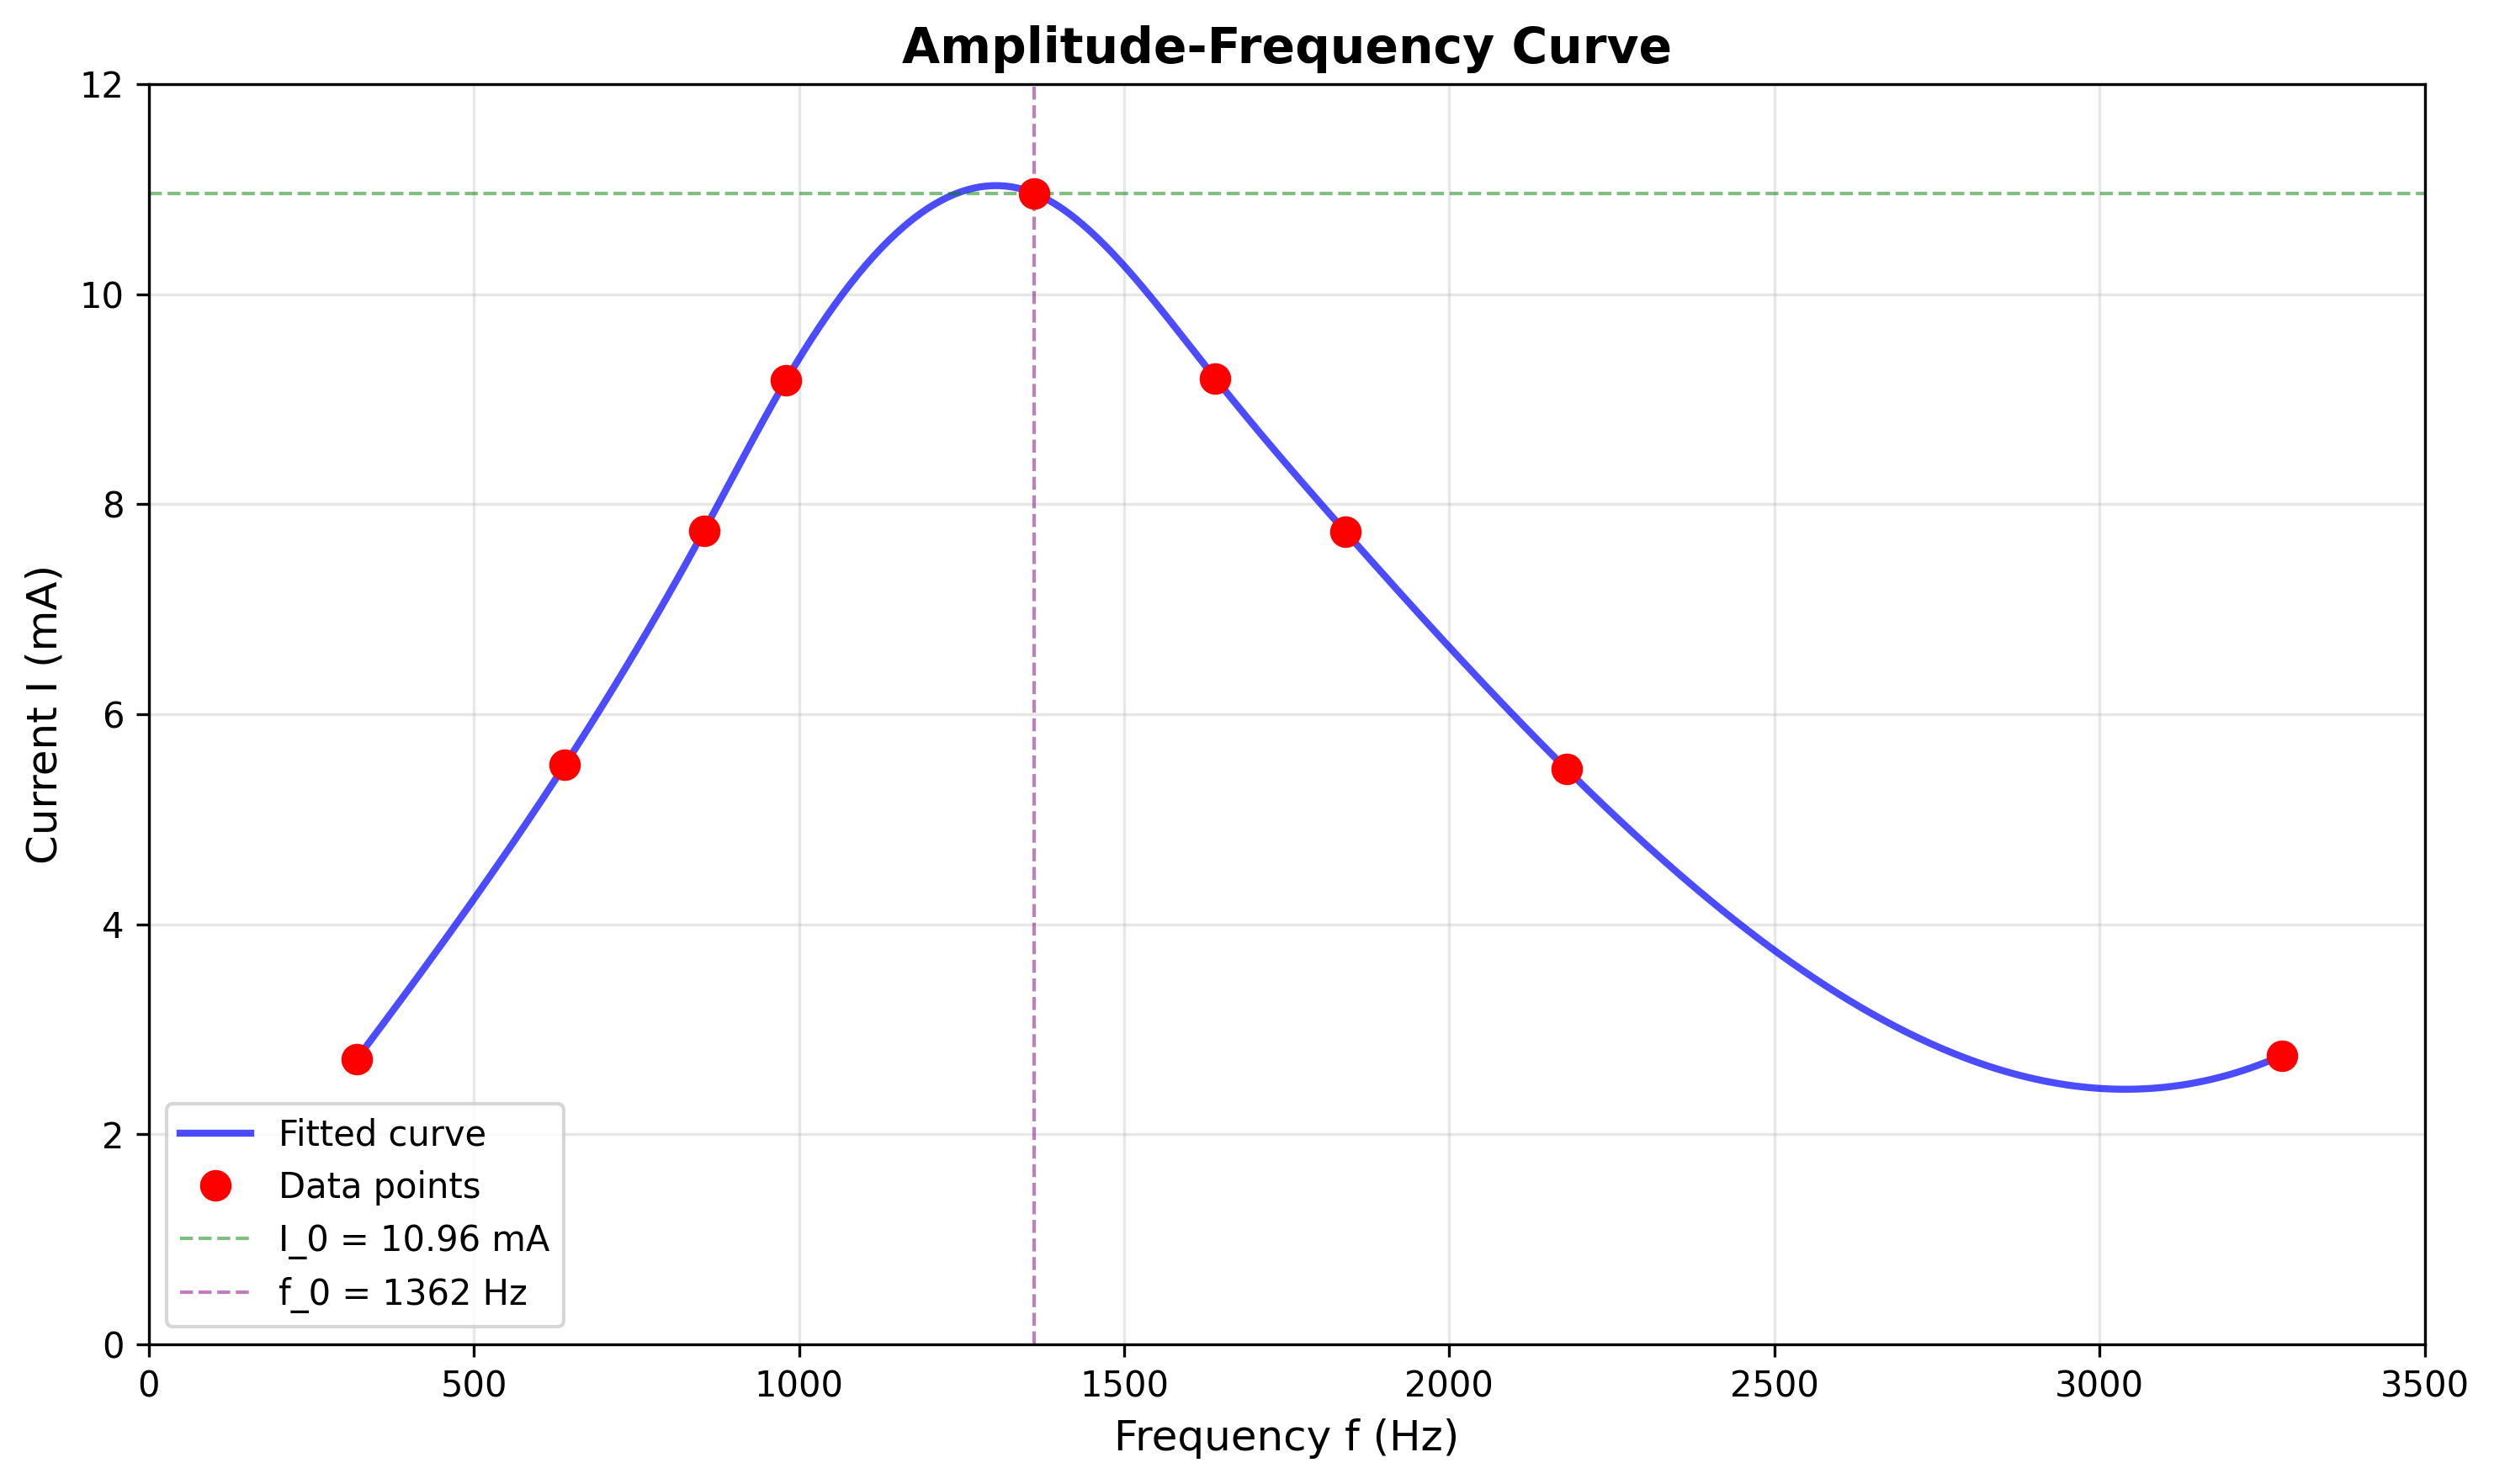
\includegraphics[width=0.8\textwidth]{../picture/amplitude_frequency.png}
        \caption{幅频特性曲线}
    \end{figure}

\textbf{数据分析：}
\begin{itemize}[label={}]
    \item 由实验数据表格：上限截止频率$f_{h2} = 1840 Hz$，下限截止频率$f_{l2} = 854 Hz$，谐振频率$f_{hc} = 1362 Hz$。

    \item 计算品质因数理论值：
    \begin{equation*}
    Q = \dfrac{\omega_0 L}{R + R_L} = \dfrac{2\pi \times 1362 \times 0.1}{510 + 135} = 1.32
    \end{equation*}

    \item 由测量结果，功率因数的实际值：
    \begin{equation*}
    Q = \dfrac{f_{hc}}{f_{h2} - f_{l2}} = \dfrac{1362}{1840 - 854} = 1.38
    \end{equation*}
    
    \item 相对误差：
    \begin{equation*}
    U_r(Q) = \dfrac{\lvert Q_{measured} - Q_{theoretical} \rvert}{Q_{theoretical}} \times 100\% = \dfrac{\lvert 1.38 - 1.32 \rvert}{1.32} \times 100\% = 4.55\%
    \end{equation*}

    \item 由计算结果可知，相对误差较小，测量结果准确。
        \begin{figure}[H]
        \centering
        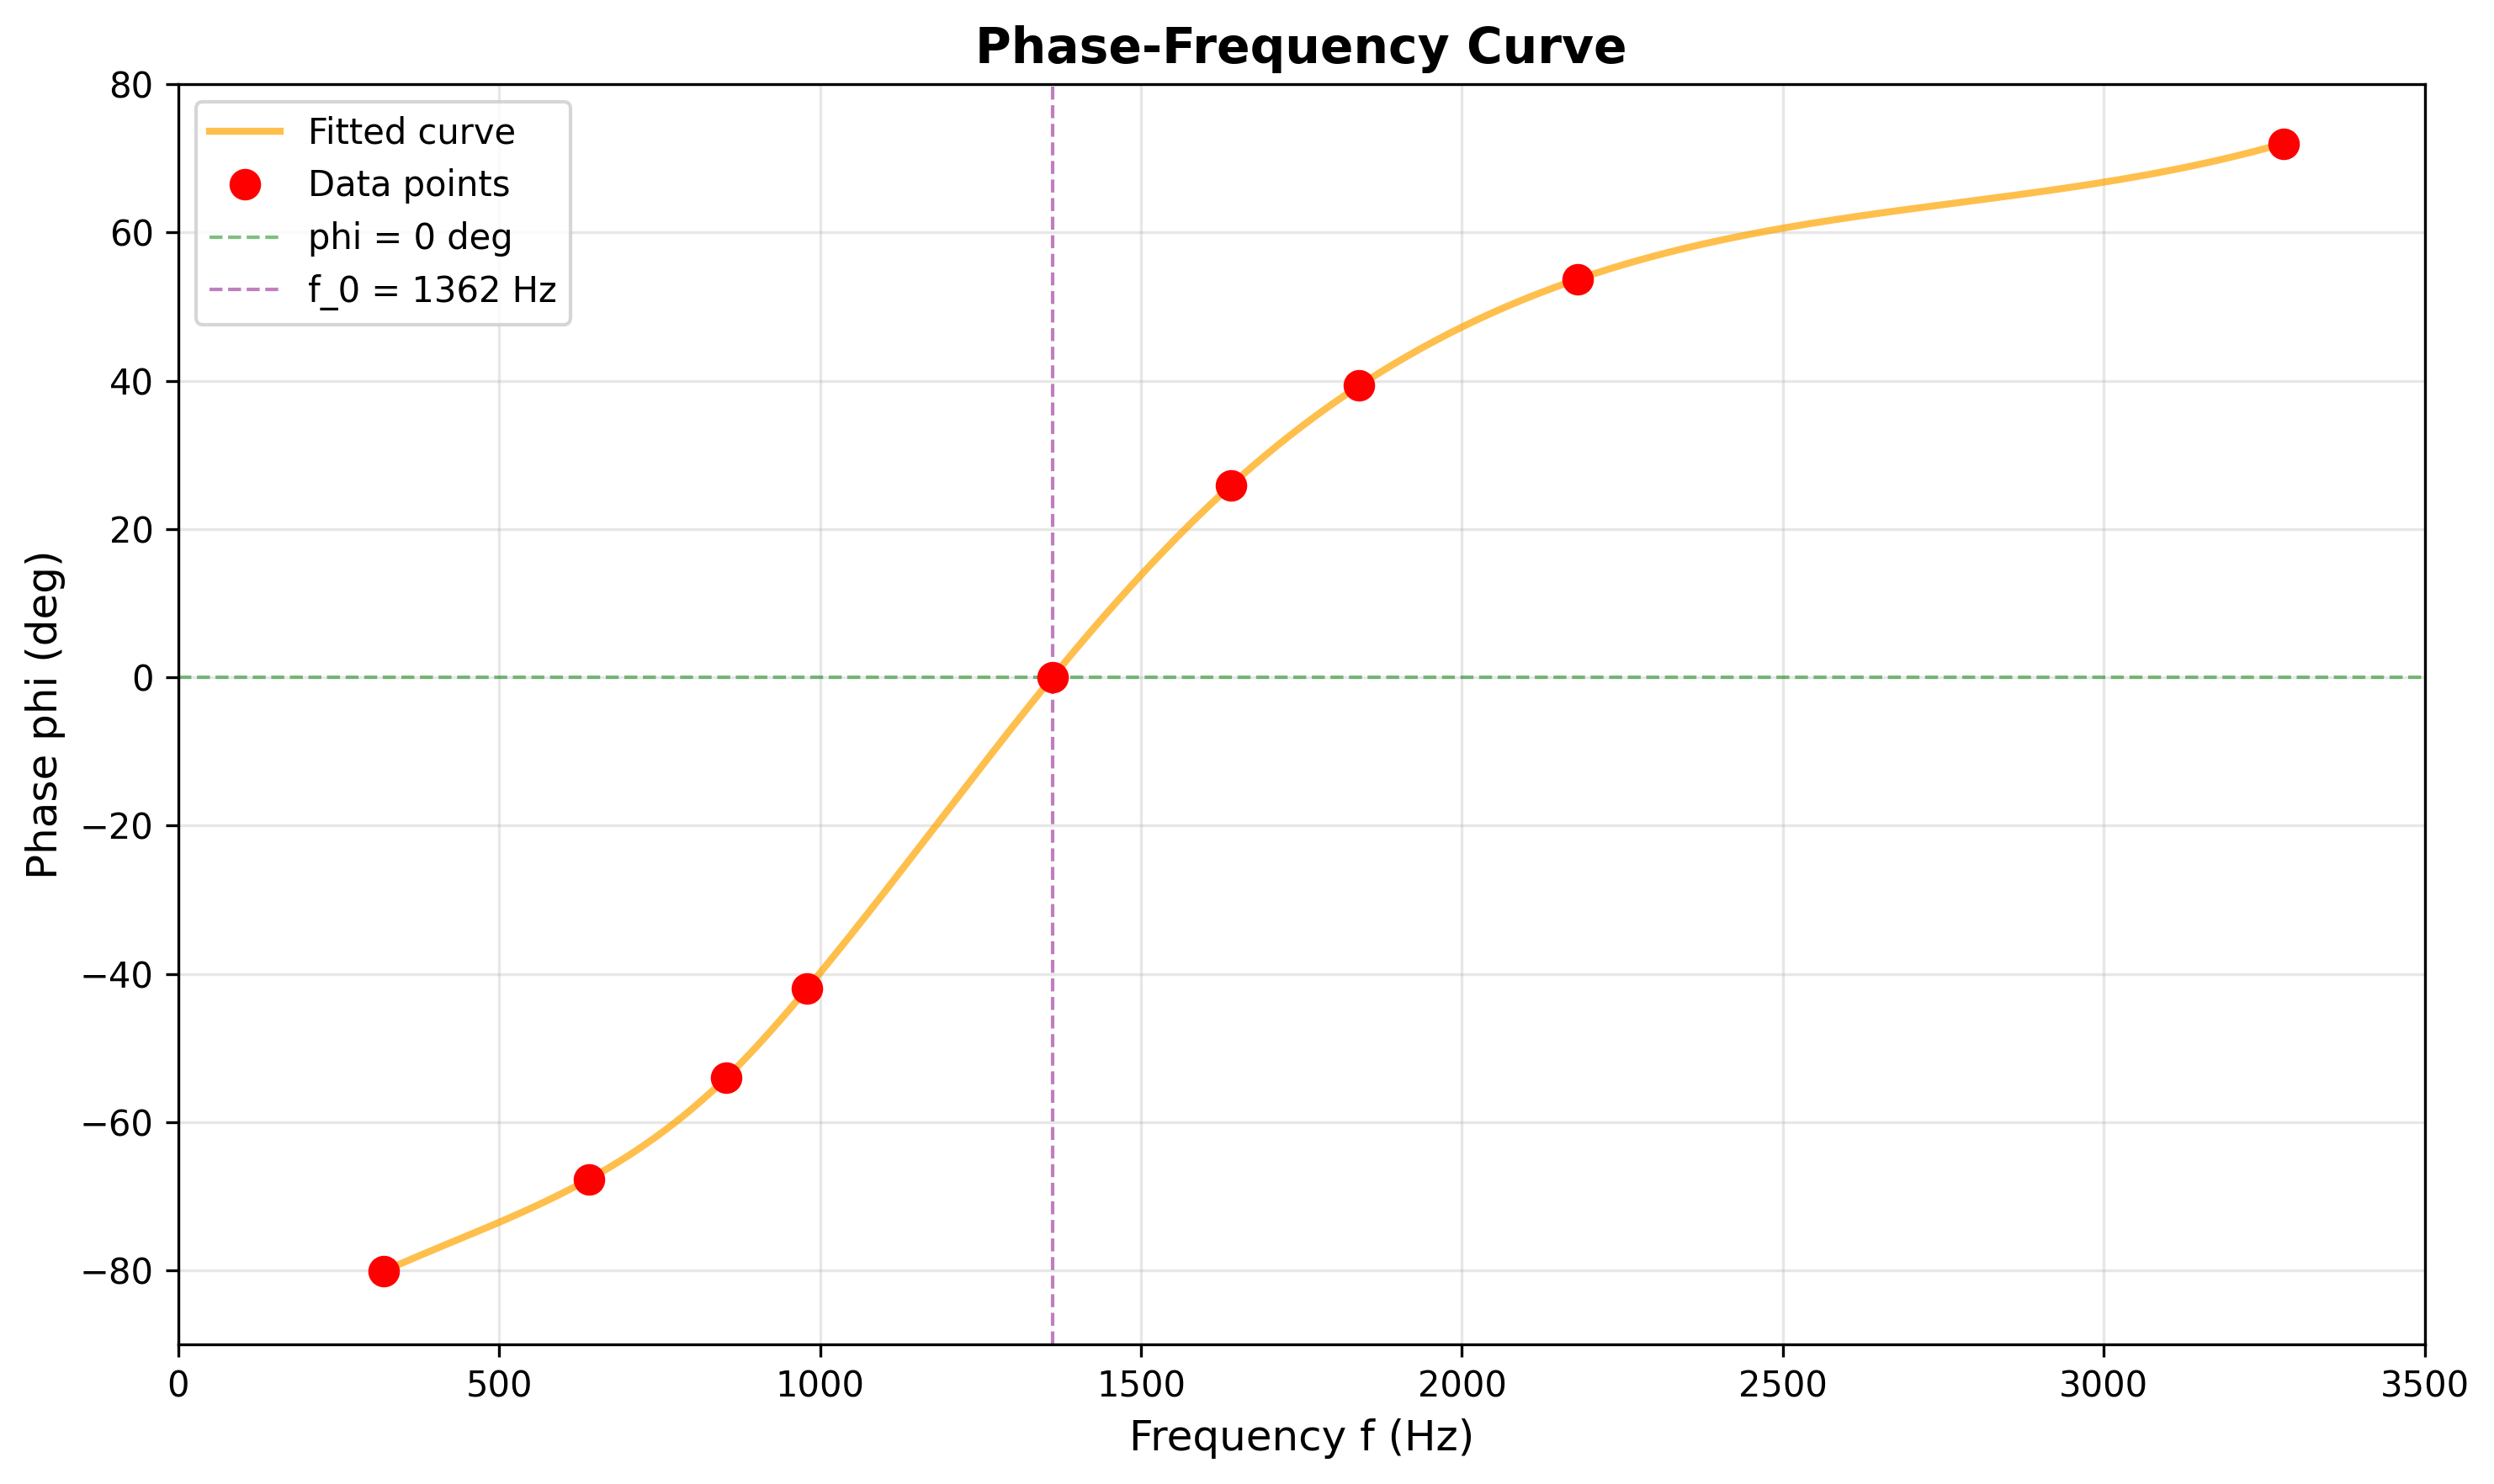
\includegraphics[width=0.8\textwidth]{../picture/phase_frequency.png}
        \caption{相频特性曲线}
    \end{figure}
    
\end{itemize}



\section*{六、实验小结}
通过本次串联谐振实验,加深了对串联谐振条件和特点的理解。实验中测量了RLC串联谐振电路的幅频特性和相频特性,绘制了相应的频率响应曲线,从实际数据和实验过程中深入理解了RLC电路的频率特性规律。掌握了运用示波器观察波形、测量电压电流相位关系等多种方法来判断电路是否达到谐振状态。实验结果表明,当电路谐振时,电流达到最大值,且电压与电流同相位,验证了理论分析的正确性。通过改变电路参数观察品质因数Q对谐振特性的影响,进一步加深了对谐振电路性能的认识。

\end{document}